\documentclass[tikz]{standalone}

\usepackage{tikz} % Graph drawing
\usetikzlibrary{graphs} 

\makeatletter
\@ifundefined{mynode} 
    {\def\mynode {\node[circle, draw=black, fill=black, inner sep=2pt, minimum size=3pt]}}
    {}
\makeatother

\begin{document}
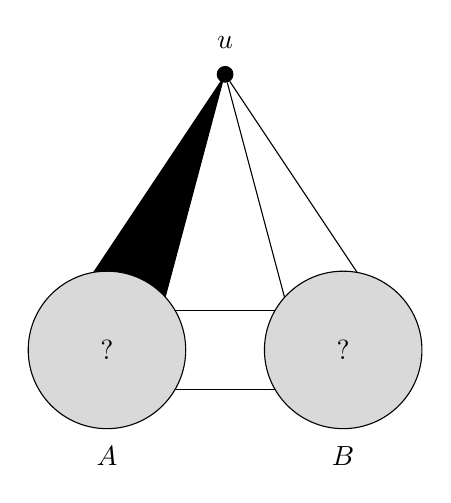
\begin{tikzpicture}
    \mynode (v1) at (0, 1) {};
    \node (v2) at (1.2, 1) {};
    \node (v3) at (2.8, 1) {};
    \node (v4) at (4, 1) {};
    \node (v5) at (1, 0) {};
    \node (v6) at (3, 0) {};
    \mynode (u) at (2, 4) {};
    \node (c1) at (0.5, 0.5) {};
    \node (c2) at (3.5, 0.5) {};

    \draw (v3) -- (v2);
    \draw (v5) -- (v6);
    \draw (u) -- (v3);
    \draw (u) -- (v4);

    \fill[fill=black] (u.center) -- (v1.center) -- (v2.center);

    % Draw the circles with a light grey background
    \filldraw[fill=gray!30, draw=black, solid] (c1) circle [radius=1];
    \filldraw[fill=gray!30, draw=black, solid] (c2) circle [radius=1];
    \node at (c1) [] {$?$};
    \node at (c2) [] {$?$};

    % Label everything
    \node at (u) [above = 0.2cm] {$u$};
    \node at (c1) [below = 1.1cm] {$A$};
    \node at (c2) [below = 1.1cm] {$B$};
\end{tikzpicture}
\end{document}